\section{Manipulation 1 "Mesurer la vitesse de propagation du son dans des
barreaux solides par méthode de résonance en mode continu."}
\subsection{\large Approches / Méthodes}
\subsubsection{\large Rappels Théoriques}

\paragraph{Introduction}

\begin{figure}[h]
    \centering
    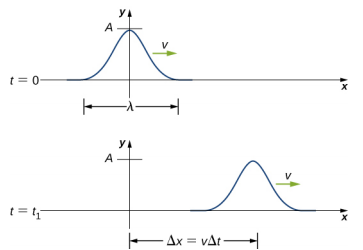
\includegraphics[width=10cm]{png/onde.png}
    \caption{Onde progressive à une dimension.~\cite{image-onde-progressive}}
\end{figure}

\paragraph{Equations physiques}
ok
\begin{figure}[h]
    \centering
    \begin{minipage}{0.45\textwidth}
        \centering
        \adjustbox{max width=\linewidth}{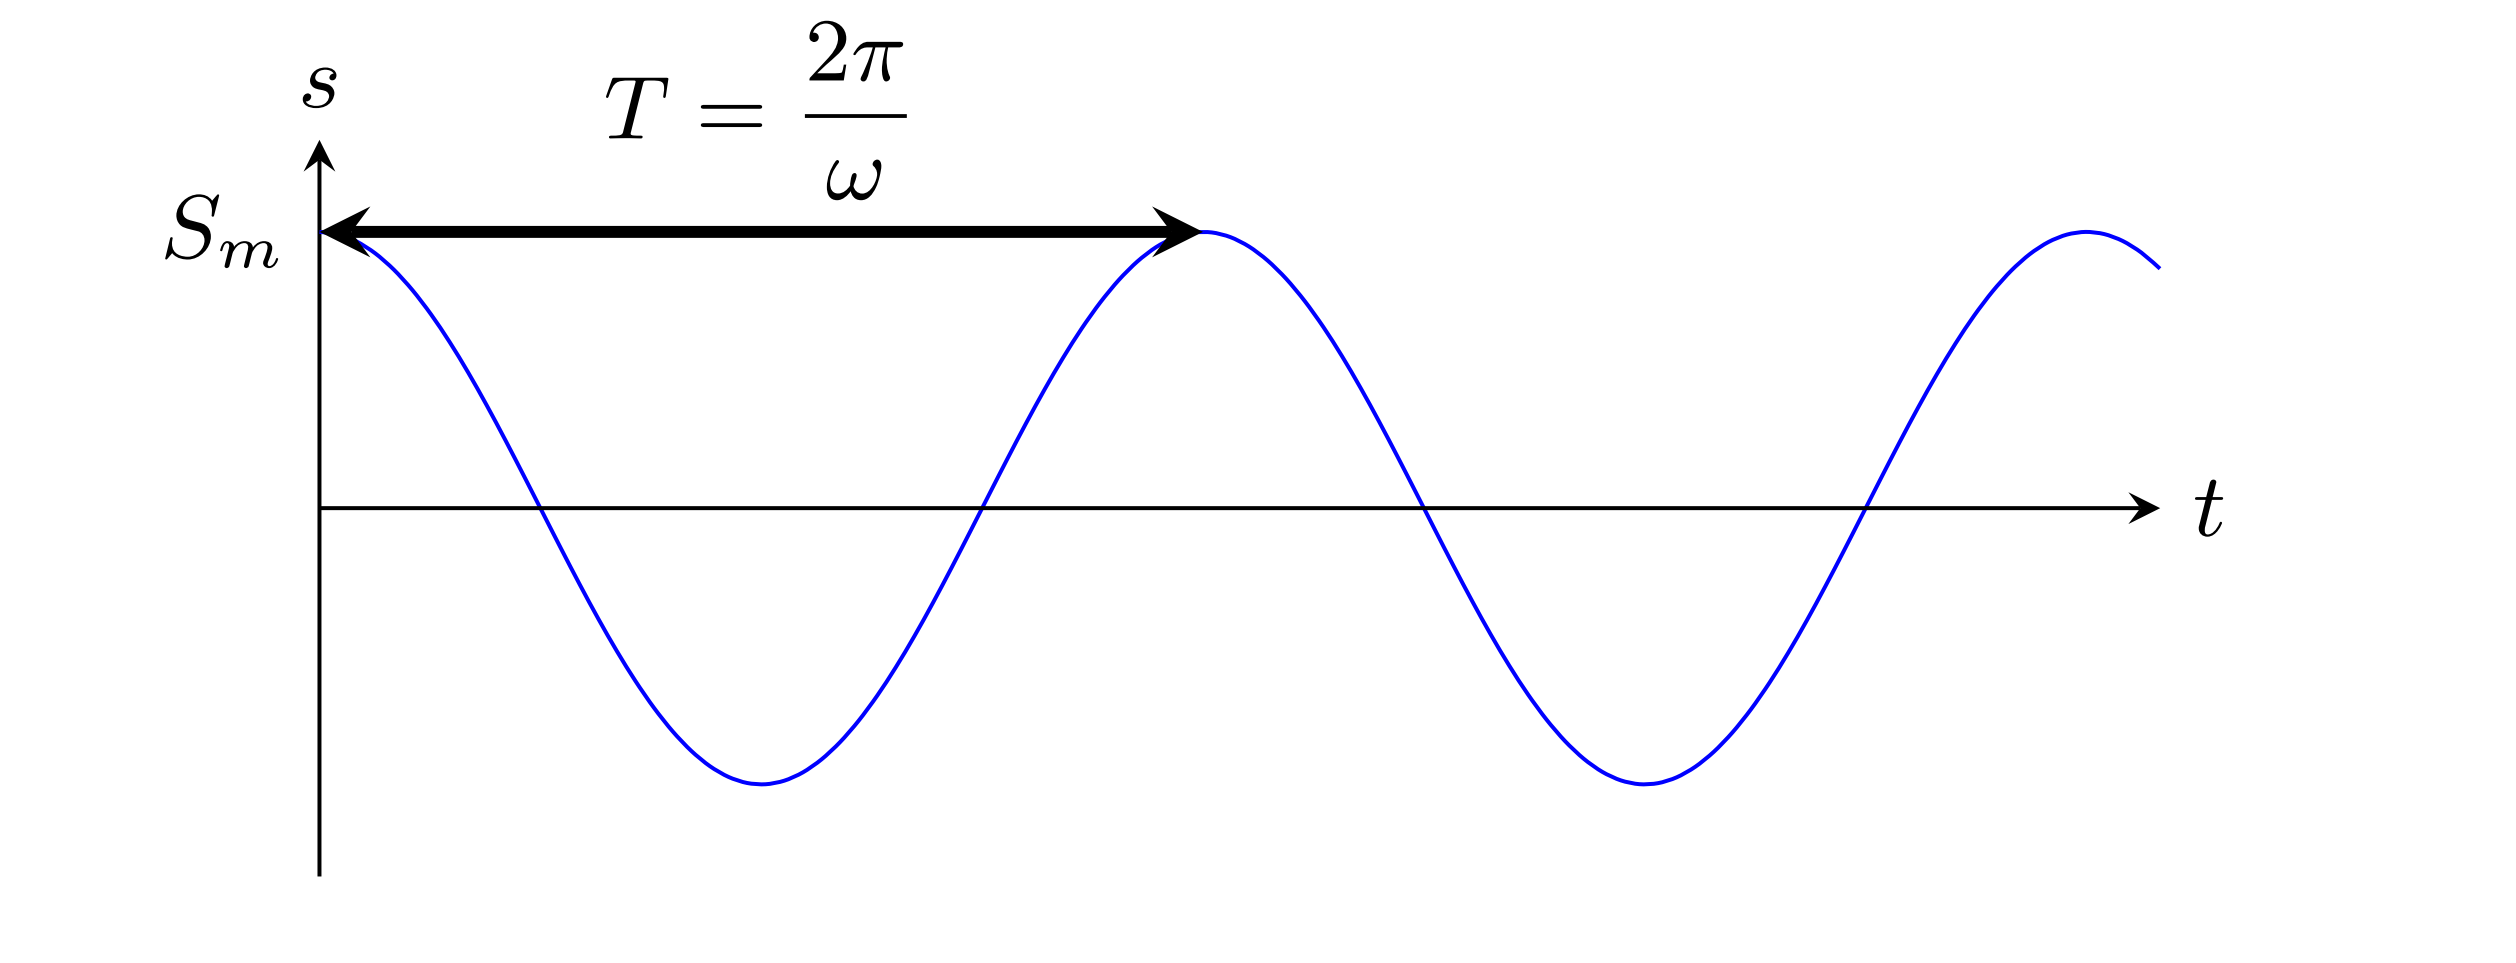
\includegraphics{png/evolution_temporelle.png}}
        \caption{Evolution temporelle d'un point donné du milieu.~\cite{propagation-onde}}
    \end{minipage}
    \hfill
    \begin{minipage}{0.45\textwidth}
        \centering
        \adjustbox{max width=\linewidth}{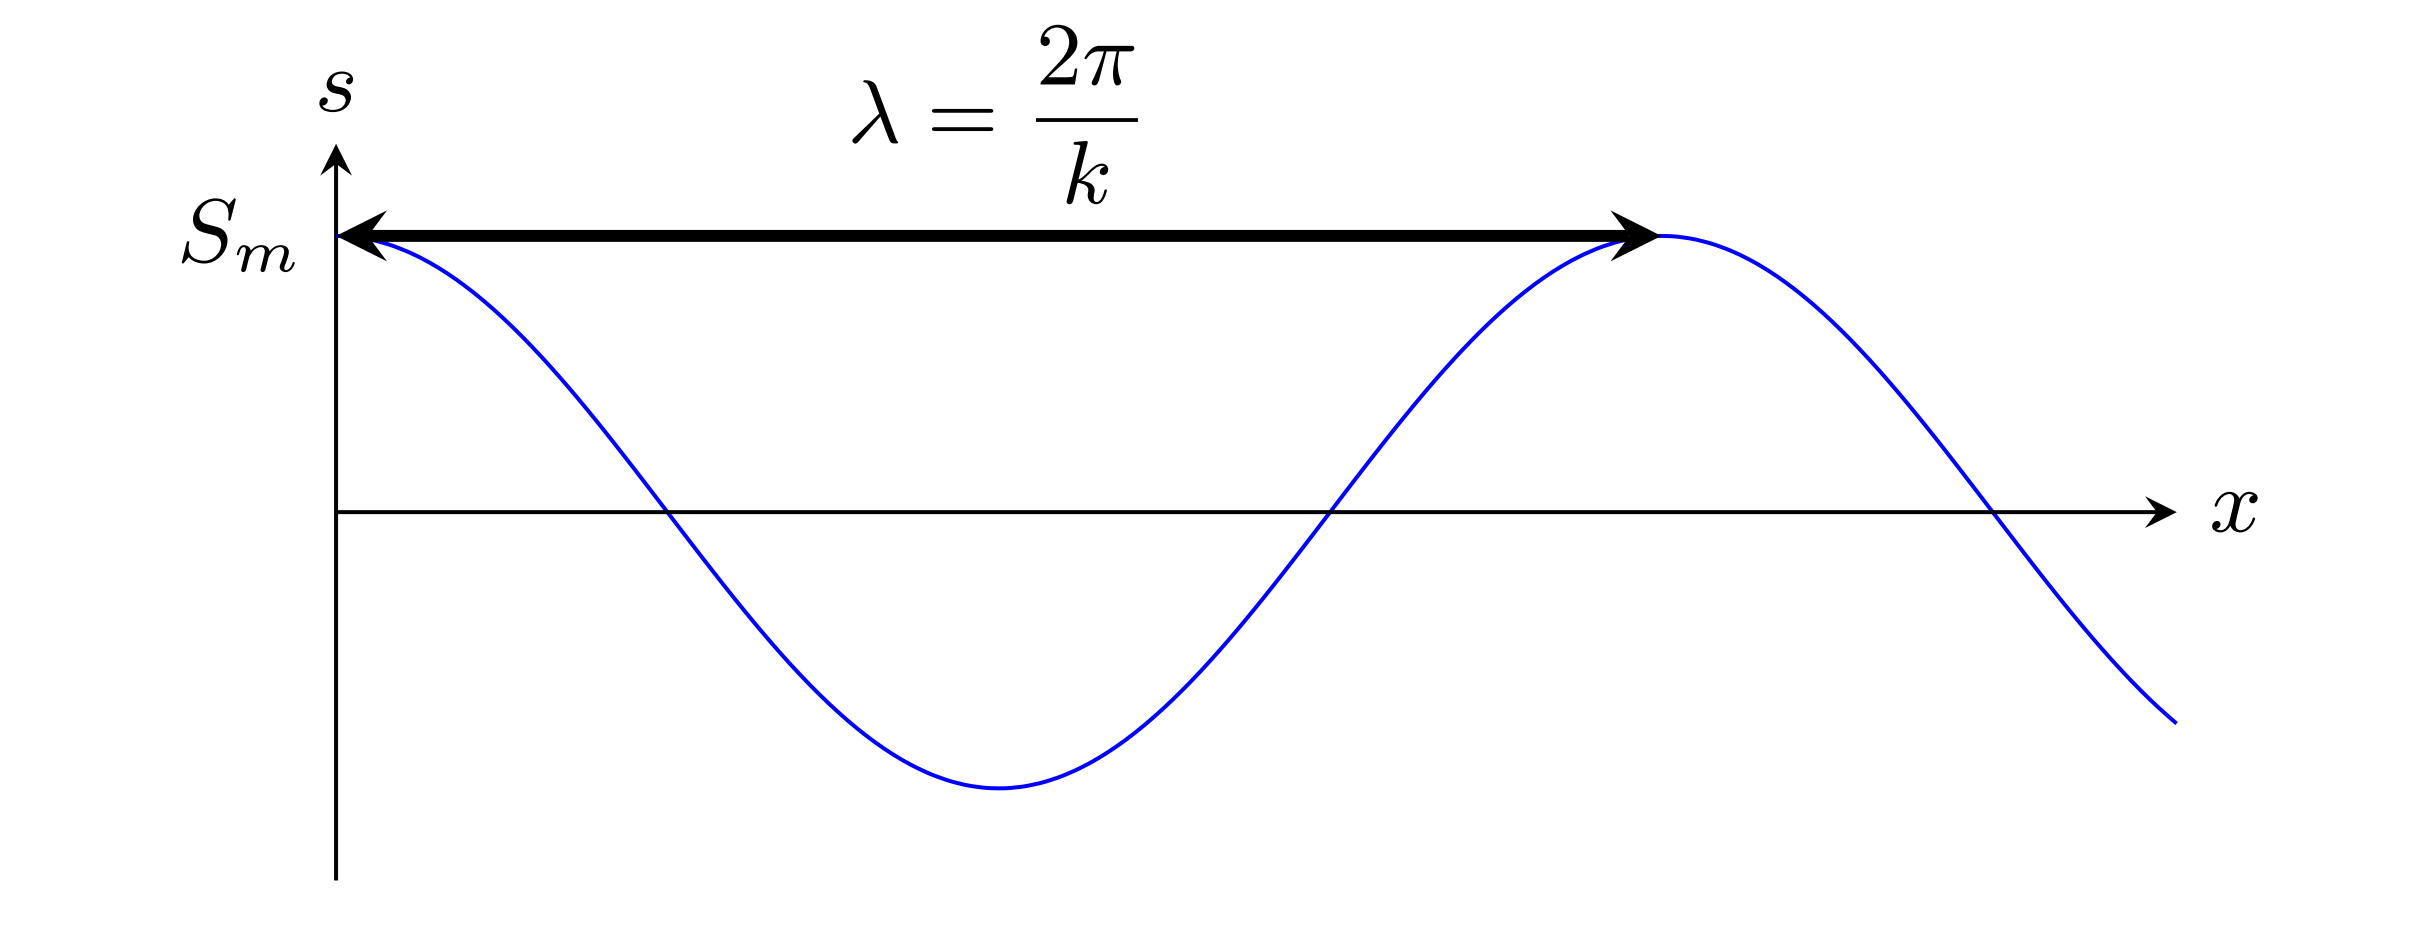
\includegraphics{png/evolution_spatiale.png}}
        \caption{Evolution spatiale du milieu à un instant donné.~\cite{propagation-onde}}
    \end{minipage}
\end{figure}

\paragraph{Calculs d'incertitudes}
La propagation d'incertitude basée sur le cours IPH est calculé de la manière 
suivante :~\cite{gravier-laurent}\\[2ex]
Relation :
\begin{align}
    g &= f(a) \\
    \Delta g &= |\frac{\partial f}{\partial a}|\Delta a + |\frac{\partial f}{\partial b}|\Delta b + |\frac{\partial f}{\partial c}|\Delta c + \ldots
\end{align}
L'incertitude $\Delta g$ est arrondi à 1 chiffre significatif selon le cours 
IPH.\\[2ex]
a, b, c sont les grandeurs physiques mesurées de manière directe. \\[2ex]
$\Delta a, \Delta b, \Delta c$ sont les incertitudes absolues des grandeurs 
a,b,c.\\[2ex]
$|\frac{\partial f}{\partial a}|;|\frac{\partial f}{\partial b}|;|\frac{\partial f}{\partial c}|$
sont les dérivées partielles de B par rapport à a, b, c.\\
\begin{align}
    \shortintertext{ Dans notre cas, la première méthode de mesure 
    nous donne une incertitude:}\notag\\
    \Delta c &= c \left( \frac{\Delta x}{x} + \frac{\Delta t}{t} \right) \\[2ex]
    \shortintertext{ $\Delta x$ $\pm$ 2 mm (valeur à ajuster)}
    \shortintertext{ $\Delta t$ $\pm$ 500 ms (valeur à ajuster)}\notag \\
    \shortintertext{ La deuxième méthode de mesure nous donne 
    une incertitude:}\notag  \\
    \Delta c &= c \left( \frac{\Delta \lambda}{\lambda} + \frac{\Delta f}{f} \right) \\[2ex] \notag 
    \shortintertext{ $\Delta \lambda$ $\pm$ 1 mm (valeur à ajuster)}
    \shortintertext{ $\Delta f$ $\pm$ 5 Hz (valeur à ajuster)} \notag
    \shortintertext{ L'équation (14) nous donne une incertitude:}
    \Delta c &= \frac{c}{2} \left( \frac{\Delta E}{E} + \frac{\Delta \rho}{\rho} \right)
    \shortintertext{ $\Delta E$ $\pm$ 10 $GPa$ (valeur à ajuster, sera prise d'internet)}
    \shortintertext{ $\Delta \rho$ $\pm$ 2 $\frac{kg}{m^3}$ (valeur à ajuster, sera prise d'internet)} \notag
    \shortintertext{ L'équation (15) nous donne une incertitude:}
    \Delta f &= f \left( \frac{\Delta c}{c} + \frac{\Delta d}{d} \right) \\[2ex]
    \shortintertext{ $\Delta c$ $\pm$ 2 $\frac{m}{s^2}$ (valeur à ajuster)}
    \shortintertext{ $\Delta d$ $\pm$ 1 mm (valeur à ajuster)}\notag \\
\end{align}

\newpage

\subsubsection{\large Protocole expérimental}
\paragraph{Présentation du montage}